\documentclass[11pt,wide]{article}

\usepackage{polski}
\usepackage[utf8]{inputenc}

\usepackage{graphicx} 

\usepackage{mathtools}
\usepackage{amsthm}
\usepackage{verbatim}
\usepackage{xcolor}

\usepackage{hyperref}


\hypersetup{
    colorlinks=true,
    linkcolor=blue,
    filecolor=magenta,      
    urlcolor=cyan,
    citecolor=green,
    pdftitle={Sharelatex Example},
    bookmarks=true,
}

\newcommand\numeq[1]%
  {\stackrel{\scriptscriptstyle \mkern-1.5mu#1\mkern-1.5mu }{=}}

\newtheorem{thm}{Twierdzenie}
\newtheorem{remark}{Uwaga}
\newtheorem{lemat}{Lemat}
\newtheorem{wniosek}{Wniosek}
\newtheorem{definicja}{Definicja}
\newtheorem{ciekawostka}{Ciekawostka}
\newtheorem{przyklad}{Przykład}

% Marginesy
\topmargin=-0.45in
\evensidemargin=0in
\oddsidemargin=0in
\textwidth=6.5in
\textheight=9.0in
\headsep=0.25in

\title{Analiza numeryczna (M) - Pracownia 1 \\ Zadanie P1.8\\
Analiza i wyliczanie przybliżonych wartości elementów ciągu}
\date{Wrocław, Październik 30, 2019}
\author{Jakub Kuciński, prowadzący Witold Karczewski}

\begin{document}

\maketitle
\thispagestyle{empty} 
\tableofcontents

\section{Wprowadzenie}
Obliczanie wartości wyrazów ciągu jest jendym z podstawowych zagadnień metod numerycznych. Można spotkać się z problemem obliczania wyrazów ciągu o elementach jawnej postać lub też ciągu o elementach spełniających pewną zależność rekurencyjną. W każdym przypadku wybór metody zależy ściśle od rodzaju ciągu, z którym mamy do czynienia, jego własności oraz wzoru, którym jest opisany. Celem tego sprawozdania jest zbadanie własności ciągu \(\displaystyle y_n = \int_0^1 t^n e^t \mathrm{dt}\) oraz próba jak najdokładniejszego wyliczenia wartości jego pierwszych 20 wyrazów, a także stwierdzenie źródła niedokładności i dokładności zastosowanych metod.
\section{Twierdzenia wykorzystane w sprawozdaniu}
\begin{thm} \label{tw:sumacalek}
Jeżeli funkcje f i g są całkowalne na przedziale \([a,b]\) to funkcje \(f(x) \pm g(x)\) też są całkowalne oraz
\begin{equation} 
\int_a^b f(x)\mathrm{dx} \pm \int_a^b g(x)\mathrm{dx} = \int_a^b (f(x) \pm g(x))\mathrm{dx}
\end{equation}
\end{thm}
\begin{proof}
Przedstawiony w \cite{Paluszynski}, strona 135.
\end{proof}

\begin{thm} \label{tw:greeq}
Jeżeli funkcje f i g są całkowalne na przedziale \([a,b]\) i dla wszystkich \(x \in [a,b]\) mamy \(f(x) \leq g(x)\) to
\begin{equation} 
 \int_a^b f(x)\mathrm{dx} \leq \int_a^b g(x)\mathrm{dx}
\end{equation}
Jeśli dodatkowo  \(f(x) < g(x)\) poza skończoną liczbą argumentów z przedziału \([a,b]\) to 
\begin{equation} 
\int_a^b f(x)\mathrm{dx} < \int_a^b g(x)\mathrm{dx}
\end{equation}
\end{thm}
\begin{proof}
Przedstawiony w \cite{Paluszynski}, strona 136.
\end{proof}

\begin{thm} \label{tw:ztrric}
Zasadnicze twierdzenie rachunku różniczkowego i całkowego.\\
Jeśli funkcja \(f(x)\) jest całkowalna na \([a,b]\) oraz \(F(x)\) jest funkcją pierwotną do \(f(x)\), to
\begin{equation} 
\int_a^b f(x)\mathrm{dx} = F(b) - F(a) = F(x) \Big|_{a}^{b}
\end{equation}
\end{thm}
\begin{proof}
Przedstawiony w \cite{Szwarc}, strona 113.
\end{proof}

\begin{thm} \label{tw:czesci}
Całkowanie przez części. \\
Jeżeli funkcje f i g są ciągłe oraz \(f'~i~g' \) są całkowalne na przedziale \([a,b]\), to
\begin{equation} 
\int_a^b f'(x)g(x) \mathrm{dx} = f(x)g(x)\Big|_{a}^{b} - \int_a^b f(x)g'(x) \mathrm{dx}
\end{equation}
\end{thm}
\begin{proof}
Wiemy, że \( (f(x)g(x))' = f'(x)g(x) + f(x)g'(x)\). Z zasadniczego twierdzenia rachunku różniczkowego i całkowego \eqref{tw:ztrric} otrzymujemy:
\begin{equation} 
f(x)g(x)\Big|_{a}^{b} = \int_a^b (f'(x)g(x) + f(x)g'(x)) \mathrm{dx} \numeq{\eqref{tw:sumacalek}} \int_a^b f'(x)g(x) \mathrm{dx}
+ \int_a^b f(x)g'(x) \mathrm{dx}
\end{equation}
Po odpowiednium uporządkowaniu elementów dostajemy tezę.
\end{proof}

\begin{thm} \label{tw:wartsred}
Twierdzenie o wartości średniej.\\
Jeśli funkcje f i g są całkowalne na \([a,b]\), \(g(x) \geq ­0\) dla \(x \in [a,b]\) oraz \(m \leq f(x) \leq M\) dla \(x \in [a,b]\) to
\begin{equation} 
\int_a^b f(x)g(x) \mathrm{dx} = \lambda \int_a^b g(x) \mathrm{dx}
\end{equation}
gdzie \(\lambda \in [m, M]\).
\end{thm}
\begin{proof}
Przedstawiony w \cite{Szwarc}, strona 118.
\end{proof}

\begin{thm} \label{tw:otrzechciagach}
Twierdzenie o 3 ciągach.\\
Jeśli ciągi \(a_n, b_n, c_n\) spełniają \(a_n \leq b_n \leq c_n \) oraz \(\lim_{n\to \infty}a_n = \lim_{n\to \infty}b_n = g\) to
\begin{equation} 
\lim_{n\to \infty}c_n = g
\end{equation}
\end{thm}
\begin{proof}
Przedstawiony w \cite{Paluszynski}, strona 38.
\end{proof}

\section{Własności ciągu \(\{y_n\}\)}
\subsection{Monotoniczność} \label{wl:malejacy}
W celu zbadania monotoniczności ciągu \(\displaystyle y_n = \int_0^1 t^n e^t \mathrm{dt}\) przeanalizujemy różnicę dwóch kolejnych wyrazów tego ciągu:
\begin{equation}
y_n - y_{n+1} = \int_0^1 t^n e^t \mathrm{dt} - \int_0^1 t^{n+1} e^t \mathrm{dt} \numeq{\eqref{tw:sumacalek}} 
\int_0^1 (t^n e^t - t^{n+1} e^t) \mathrm{dt} = \int_0^1 t^n e^t(1 - t)\mathrm{dt}
\end{equation}
Zauważmy, że wyrażenie podcałkowe \(t^n e^t(1 - t)\) dla \( t \in (0, 1) \) przyjmuje wartości dodatnie oraz dla 
\(t=1\) i~\(t=0\) jest równe 0.  Stąd z twierdzenia \eqref{tw:greeq} otrzymujemy: 
\begin{equation}
0 = \int_0^1 0 \cdot  \mathrm{dt} < \int_0^1 t^n e^t(1 - t)\mathrm{dt}
= y_n - y_{n+1}
\end{equation} 
Zatem \(y_n - y_{n+1} > 0 \), czyli ciąg \(\{y_n\}\) jest ściśle malejący.

\subsection{Ograniczenia górne i dolne na wyrazy ciągu} \label{wl:ograniczenia}
Niech \(f(t) = e^t\) oraz \(g(t) = t^n\). Wtedy f i g są całkowalne na \([a,b]\), \(g(t) \geq ­0\) dla \(t \in [0,1]\) oraz \(1 \leq f(t) \leq e\) dla \(t \in [0,1]\), bo \(f(t)\) ściśle rosnąca i ciągła na \([0,1]\) (\(f(0) = 1\) oraz \(f(1) = e\)). Zatem z twierdzenia o wartości średniej \eqref{tw:wartsred} otrzymujemy:
\begin{align} 
1\int_0^1 g(t) \mathrm{dt} \leq \int_0^1 f(t) & g(t) \mathrm{dt} \leq e \int_0^1 g(t) \mathrm{dt} \\
\int_0^1 t^n \mathrm{dt} \leq \int_0^1 f(t) & g(t) \mathrm{dt} \leq e \int_0^1 t^n \mathrm{dt} \\
\frac{t^{n+1}}{n+1}\Big|_{0}^{1} \leq \int_0^1 f(t) & g(t) \mathrm{dt} \leq e \frac{t^{n+1}}{n+1}\Big|_{0}^{1} \\
\frac{1}{n+1} \leq \int_0^1 f(t) & g(t) \mathrm{dt} \leq \frac{e}{n+1} 
\end{align}
Otrzymaliśmy więc ograniczenie na wyrazy ciągu \(\{y_n\}\)
\begin{equation}\
\frac{1}{n+1} \leq \; y_n \leq \frac{e}{n+1}
\end{equation}

\subsection{Zbieżność}
Pokażemy zbieżność ciągu \(\{y_n\}\) do zera.
Przypomnijmy udowodnione w poprzednim podrozdziale nierówności:
\begin{equation}
\frac{1}{n+1} \leq \; y_n \leq \frac{e}{n+1}
\end{equation}
Zauważmy, że 
\begin{equation}
\lim_{n\to \infty}\frac{1}{n+1} = \lim_{n\to \infty}\frac{e}{n+1} = 0
\end{equation}
Zatem z twierdzenia o trzech ciągach dostajmy 
\begin{equation}
\lim_{n\to \infty}y_n = 0
\end{equation}


\subsection{Zależność rekurencyjna wyrazów ciągu}
Pokażemy, że między kolejnymi elementami ciągu \(\{y_n\}\) zachodzi następujący związek rekurencyjny:
\begin{equation} \label{tw:zalrek}
y_{n+1} = e - (n+1)y_n
\end{equation}
W tym celu przekształcimy wzór na \(y_{n+1}\) przy użyciu twierdzenia o całkowaniu przez części \eqref{tw:czesci}:

\begin{multline}
y_{n+1} = \int_0^1 t^{n+1} e^t\mathrm{dt} =  \int_0^1 t^{n+1} (e^t)'\mathrm{dt}\numeq{\eqref{tw:czesci}} 
t^{n+1}e^t \Big|_{0}^{1} - \int_0^1 (t^{n+1})' e^t\mathrm{dt} = \\ = 1^{n+1}e^1 - 0^{n+1}e^0 - \int_0^1 (n+1)t^n e^t\mathrm{dt}
= e - (n+1)\int_0^1 t^n e^t\mathrm{dt} = e - (n+1)y_n
\end{multline}

\section{I metoda: wyliczanie kolejnych elementów ciągu przy użyciu zależności rekurencyjnej}
Wyliczmy wartość początkową \(y_0\) bezpośrednio ze wzoru ciągu \(\{y_n\}\), a następnie korzystając z tego wyniku wyrazy
\(y_1, y_2, \dots ,y_{20} \).
\begin{equation}
y_0 = \int_0^1 t^0 e^t\mathrm{dt} = \int_0^1 e^t\mathrm{dt} = e^t\Big|_{0}^{1} = e - 1
\end{equation}

\begin{comment}
Poniżej znajduje się przykładowa implementacja programu obliczającego kolejne wyrazy ciągu \(\{y_n\}\) korzystającego z~zależności rekurencyjnej w języku Julia.
\begin{verbatim}
nastepny = zeros(Float64, 20)
e = Base.MathConstants.e
nastepny[1] = e - (e - 1)
i = 2
while i <= 20
    nastepny[i] = e - i * nastepny[i-1]
    i += 1
end
\end{verbatim}
\end{comment}

\begin{figure}[h!]
Przedstawmy uzyskane wartości w porównaniu do wyników podanych przez Wolfram Alpha.
\begin{center}
  \begin{tabular}{ | c | l | l | }
  \hline
  Numer wyrazu & Wyliczone przez program & Podane przez Wolfram Alpha \\ \hline
  	1 & {\color{green}1.0} & {\color{green}1.0}\\
	2 & {\color{green}0.718281828459045}1 & {\color{green}0.718281828459045}2 \\ 
	3 & {\color{green}0.563436343081909}8 & {\color{green}0.563436343081909}5 \\ 
	4 & {\color{green}0.46453645613140}58 & {\color{green}0.46453645613140}71\\ 
	5 & {\color{green}0.3955995478020}16 & {\color{green}0.3955995478020}096\\ 
	6 & {\color{green}0.3446845416469}4906 & {\color{green}0.3446845416469}8736\\ 
	7 & {\color{green}0.305490036930}40166 & {\color{green}0.305490036930}13366\\ 
	8 & {\color{green}0.27436153301}583177 & {\color{green}0.27436153301}79761\\ 
	9 & {\color{green}0.249028031}31655915 & {\color{green}0.249028031}29726034\\ 
	10 & {\color{green}0.228001515}29345358 & {\color{green}0.228001515}4864418\\ 
	11 & {\color{green}0.2102651}6023105568 & {\color{green}0.2102651}5810818538\\ 
	12 & {\color{green}0.1950999}0568637692 & {\color{green}0.1950999}3116082064\\ 
	13 & {\color{green}0.18198}305453614516 & {\color{green}0.18198}272336837698\\ 
	14 & {\color{green}0.1705}1906495301283 & {\color{green}0.1705}2370130176742\\ 
	15 & {\color{green}0.1604}958541638526 & {\color{green}0.1604}26308932534\\ 
	16 & {\color{green}0.15}034816183740363 & {\color{green}0.15}146088553850118\\ 
	17 & {\color{green}0.1}6236307722318344 & {\color{green}0.1}4344677430452527\\ 
	18 & -0.2042535615582568 & 0.1362398909775906\\
	19 & 6.599099498065924 & 0.12972389988482377\\
	20 & -129.26370813285942 & 0.12380383076256996\\ 
	\hline
  \end{tabular}
\end{center}
\end{figure}
\clearpage 
Zauważmy, że według obliczonych przez nasz program wartości mamy \(y_{17} > y_{16}\), chociaż według udowodnionej wcześniej monotoniczności ciągu \(\{y_n\}\) \eqref{wl:malejacy} powinniśmy dostać \(y_{17}~<~y_{16}\). Podobnie dostaliśmy, że \(y_{19} > y_{1}\). Dostaliśmy również \(y_{18},y_{20} < 0\), co jest sprzeczne z faktem \(y_n~=~\int_0^1~t^n e^t~\mathrm{dt}~>~0\). Na podstawie przeprowadzonych obliczeń można więc przypuszczać, że~wraz ze~wzrostem numeru wyliczanego elementu rośnie również niedokładność obliczeń.


\begin{figure}[h!]
Sprawdźmy, jak zachowuje się liczba dokładnych cyfr wartości wyrazów otrzymanych przez nasz program, względem wyników podanych przez Wolfram Alpha, które uznamy tutaj za wyniki dokładne.\\ \\
	\centering
	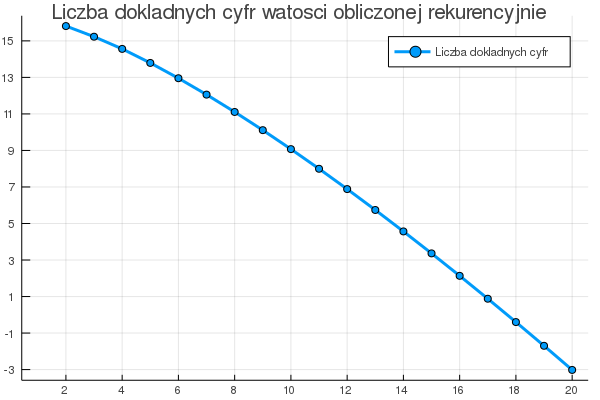
\includegraphics[width=0.82\textwidth]{plot}
\end{figure}
Na podstawie wykresu można podejrzewać, że liczba dokładnych cyfr dziesiętnych maleje nadliniowo dla kolejnych wyrazów ciągu, przy czym od wyrazu \(y_{18}\) otrzymana wartość nie ma już żadnych cyfr dokładnych.
\begin{wniosek}
Obliczanie następujących po sobie elementów \(y_0, y_1, \dots, y_{20}\) ciągu \(\{y_n\}\) przy użyciu wzoru rekurencyjnego jest niestabilne, ponieważ liczba dokładnych cyfr szybko zmniejsza się wraz z obliczaniem każdego kolejnego wyrazu.
\end{wniosek}

\section{II metoda: wyliczanie poprzednich elementów ciągu przy użyciu zależności rekurencyjnej}
Zauważmy, że wobec nierówności
\begin{equation}
\frac{1}{n+1} \leq \; y_n \leq \frac{e}{n+1}
\end{equation}
udowodnionej w \eqref{wl:ograniczenia} ciąg \(\{y_n\}\) jest wolno zbieżny, czyli wyrazy \(y_n\) i \(y_{n-1}\) są prawie sobie równe. Wtedy korzystając z własności rekurencyjnej \(y_{n} = e - n y_{n-1}\) mamy w przybliżeniu  \(y_{n} = e - ny_{n}\), a stąd 
\begin{equation}
y_{n} = \frac{e}{n+1}
\end{equation}
Przekształcając wzór rekurencyjny możemy obliczyć poprzednie wyrazy ciągu \(\{y_n\}\) korzystając z przybliżonej wartości pewnego dalszego wyrazu tego ciągu.
\begin{align} 
y_n &= e - n y_{n-1} \\
y_{n-1} &= \frac{e - y_n}{n} \label{tw:poprzednielem}
\end{align}

\begin{comment}
Poniżej znajduje się przykładowa implementacja programu w języku Julia obliczającego poprzednie wyrazy ciągu \(\{y_n\}\) korzystającego z wyżej wyliczonej zależności rekurencyjnej \eqref{tw:poprzednielem} i przybliżonej wartości dla \(y_{21}\)
\begin{verbatim}
poprzedni = zeros(Float64, 20)
e = Base.MathConstants.e
poprzedni21 = e / (21.0 + 1.0)
poprzedni[20] = (e - poprzedni21) / 21.0
i = 19
while i >=1
    poprzedni[i] = (e - poprzedni[i+1]) / (i+1)
    i -= 1
end
\end{verbatim}
\end{comment}

\begin{figure}[h!]
Przedstawmy uzyskane wartości w porównaniu do wyników podanych przez Wolfram Alpha.
\begin{center}
  \begin{tabular}{ | c | l | l | }
  \hline
  Numer wyrazu & Wyliczone przez program & Podane przez Wolfram Alpha \\ \hline
  	1 & {\color{green}1.0} & {\color{green}1.0} \\
	2 & {\color{green}0.7182818284590452} & {\color{green}0.7182818284590452} \\
	3 & {\color{green}0.5634363430819095} & {\color{green}0.5634363430819095} \\
	4 & {\color{green}0.464536456131407}04 & {\color{green}0.464536456131407}1 \\
	5 & {\color{green}0.3955995478020096} & {\color{green}0.3955995478020096} \\
	6 & {\color{green}0.3446845416469873}0 & {\color{green}0.3446845416469873}6 \\
	7 & {\color{green}0.30549003693013366} & {\color{green}0.30549003693013366} \\
	8 & {\color{green}0.274361533017976}06 & {\color{green}0.274361533017976}1 \\
	9 & {\color{green}0.2490280312972603}7 & {\color{green}0.2490280312972603}4 \\
	10 & {\color{green}0.228001515486441}43 & {\color{green}0.228001515486441}8 \\
	11 & {\color{green}0.21026515810818}938 & {\color{green}0.21026515810818}538 \\
	12 & {\color{green}0.195099931160}77226 & {\color{green}0.195099931160}82064 \\
	13 & {\color{green}0.18198272336}90055 & {\color{green}0.18198272336}837698 \\
	14 & {\color{green}0.170523701}29296804 & {\color{green}0.170523701}30176742 \\
	15 & {\color{green}0.16042630}906452457 & {\color{green}0.16042630}8932534 \\
	16 & {\color{green}0.15146088}34266519 & {\color{green}0.15146088}553850118 \\
	17 & {\color{green}0.143446}81020596278 & {\color{green}0.143446}77430452527 \\
	18 & {\color{green}0.136239}2447517153 & {\color{green}0.136239}8909775906 \\
	19 & {\color{green}0.1297}3617817645441 & {\color{green}0.1297}2389988482377 \\
	20 & {\color{green}0.123}55826492995658 & {\color{green}0.123}80383076256996 \\
	\hline
  \end{tabular}
\end{center}
\end{figure}
\clearpage
Można zauważyć, że podane przybliżenia są dokładniejsze niż w przypadku wyliczania wartości kolejnych wyrazów ciągu zaczynając od zerowego elementu. Liczbę dokładnych cyfr przedstawia wykres:
\begin{figure}[h!]
	\centering
	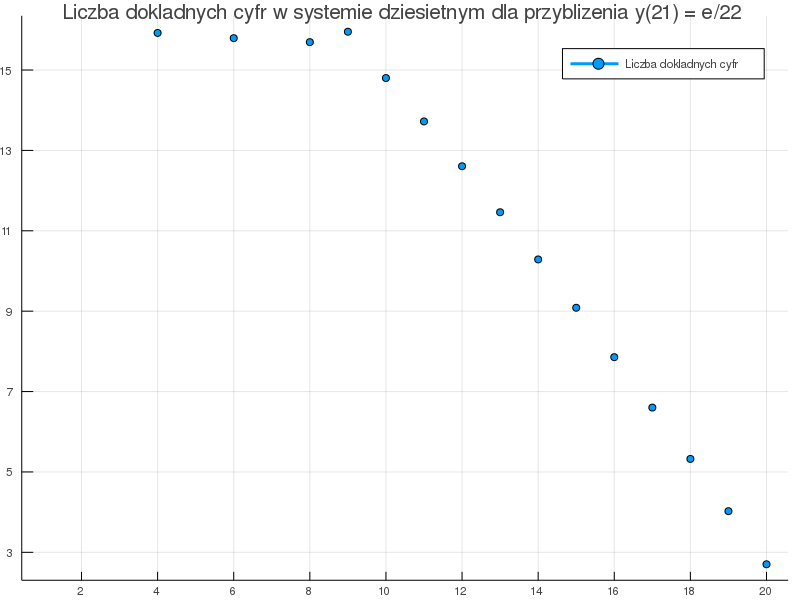
\includegraphics[width=0.82\textwidth]{plot2}
\end{figure}
\begin{remark}
Liczby całkowite, dla których na wykresie nie ma podanych wartości odpowiadają wyrazom, których wartości zostały policzone dokładnie.
\end{remark}
Z danych przedstawionych na wykresie i w tabeli można wysunąć wniosek, że wraz z obliczaniem poprzednich wyrazów, zmniejsza się błąd otrzymywanych wartości. Prawdziwe wydaje się przypuszczenie, że wraz z wyborem dalszego wyrazu jako przybliżenia początkowego, zmniejsza się błąd wyrazów początkowych. W naszym przykładzie wyrazy do \(y_9\) są dokładne/niemal dokładne. Spróbujmy osiągnąć większą dokładność początkowych 20 wyrazów, biorąc za początkowe przybliżenie \(y_{41} = \frac{e}{42}\).
\clearpage 

\begin{figure}[h!]
	\centering
	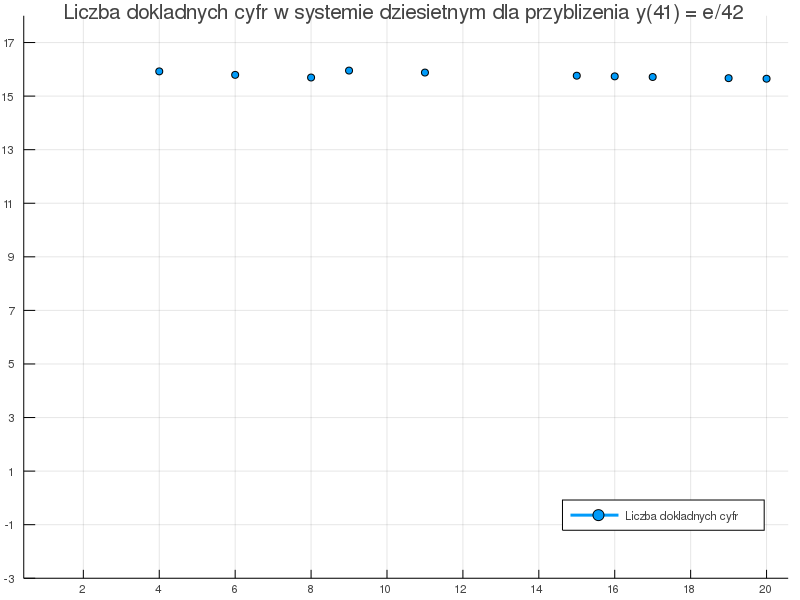
\includegraphics[width=0.82\textwidth]{plot3}
\end{figure}
Dla początkowego przybliżenia \(y_{41} = \frac{e}{42}\) otrzymaliśmy bardzo dokładne wartości (liczba cyfr dokładnych \(>\) 15) dla wszystkich pierwszych 20 wyrazów.

\section{Źródła różnicy dokładności metod I i II}
\subsection{Niedokładność metody I}
Przyjżyjmy się najpierw metodzie I, w której obliczaliśmy kolejno \(y_0, y_1, y_2, ..., y_{20}\).\\ \\
Wyraz \(y_2 = e - 2\) jest liczbą niewymierną, zatem nie może być przedstawiona w sposób dokładny w arytmetyce Float64. Niech \(\tilde{y}_2\) będzie przybliżoną wartością \(y_2\) zapisaną w arytmetyce Float64. Wtedy \(\tilde{y}_2 = y_2 \cdot (1+\epsilon)\) dla \(|\epsilon|<u\), gdzie u to precyzja arytmetyki. Załóżmy ponadto, że podstawowe działania arytmetyczne w arytmetyce Float64 wykonywane są dokładnie. Wtedy:
\begin{align*} 
\tilde{y}_3 = e - 3 \cdot \tilde{y}_2  = e - 3 \cdot y_2 \cdot (1+\epsilon) &= e - 3 y_2 - 3 \epsilon y_2 = y_3 - 3 \epsilon y_2\\ 
\tilde{y}_4 = e - 4 \cdot \tilde{y}_3 = e - 4 (y_3 - 3 \epsilon y_2) &= e - 4 y_3 + 12 \epsilon y_2 = y_4 + 12 \epsilon y_2 \\
&\cdots \\
\tilde{y}_n = e - n \cdot \tilde{y}_{n-1} = e - n (y_{n-1} \mp  \frac{1}{2} (n-1)! \epsilon \cdot y_2) &= 
e - n y_{n-1} \pm \frac{1}{2} n! \epsilon \cdot y_2 = y_n \pm \frac{1}{2} n! \epsilon \cdot y_2
\end{align*}
Mamy więc oszacowanie błędu bezwzględnego:
\begin{equation}
\Delta y_n = |\tilde{y}_n - y_n| = \frac{1}{2} n! \epsilon \cdot y_2
\end{equation}
Widać, że błąd bezwzględny rośnie niezwykle szybko wraz ze wzrostem n. Już dla n = 10 mamy:

\begin{equation}
\Delta y_{10} = \frac{1}{2} 10! \epsilon \cdot y_2 = 1. 8144 \cdot 10^{6} \cdot \epsilon \cdot y_2
\end{equation}

a dla n = 20:
\begin{equation}
\Delta y_{20} = \frac{1}{2} 20! \epsilon \cdot y_2 \simeq 1.217 \cdot 10^{18} \cdot \epsilon \cdot y_2
\end{equation}

Widzimy więc, że już dla małych wartości n błąd bezwzględny \(\Delta y_n\) staje się bardzo duży. W rzeczywistości wielkość błędu może być jeszcze większa, ze względu na niedokładność działań arytmetycznych w arytmetyce Float64 oraz przybliżoną reprezentację liczby e, których błędy również zostaną spotęgowane przez nieustanne przemnażanie przez coraz większe wartości liczby n.\\ \\

\subsection{Dokładność metody II}
Spójrzmy teraz na metodę II, w której przybliżamy pewien początkowy wyraz \(y_N\) przez \(\tilde{y}_N = \frac{e}{N+1}\), a następnie używając wzoru rekurencyjnego 
\begin{equation}
y_{n-1} = \frac{e - y_n}{n}
\end{equation}
obliczamy wartości poprzednich wyrazów ciągu. \\ \\
W \eqref{wl:ograniczenia} udowodniliśmy, że 
\begin{equation}
\frac{1}{n+1} \leq \; y_n \leq \frac{e}{n+1}
\end{equation}
Zatem \(\tilde{y}_N  = y_N (1 + \epsilon ) \), gdzie \(|\epsilon | \leq e - 1 \). Korzystając ze wzoru rekurencyjnego dostejemy:
\begin{align*}
\tilde{y}_{N-1} = \frac{e - \tilde{y}_N}{N} = \frac{e - {y}_N - \epsilon {y}_N}{N} 
&= \frac{e - {y}_N}{N} - \frac{\epsilon {y}_N}{N} = {y}_{N-1} - \frac{\epsilon \cdot {y}_N}{N} \\
\tilde{y}_{N-2} = \frac{e - \tilde{y}_{N-1}}{N-1} = \frac{e - y_{N-1} + \frac{\epsilon y_N}{N}}{N-1} 
&= \frac{e - {y}_{N-1}}{N-1} +  \frac{\epsilon y_N}{N(N-1)} = {y}_{N-2} +  \frac{\epsilon \cdot y_N}{N(N-1)}\\
&\cdots \\
\tilde{y}_k = \frac{e - \tilde{y}_{k+1}}{k+1} = \frac{e - {y}_{k+1} \mp \frac{\epsilon y_N}{ N! / (k+1)!}}{k+1} 
&= \frac{e - {y}_{k+1}}{k+1} \pm \frac{\epsilon y_N}{N!/k!} = y_{k} \pm \frac{\epsilon \cdot y_N}{N!/k!} 
\end{align*}
Mamy więc oszacowanie błędu bezwzględnego:
\begin{equation}
\Delta y_k = |\tilde{y}_k - y_k| = \frac{\epsilon \cdot y_N}{N!/k!}
\end{equation}
Widzimy więc, że im odleglejszym od wyrazu \(y_N\) jest \(y_k\) tym mnieszy będzie błąd. Zatem w celu dokładnego wyliczenia pewnej liczby początkowych elementów ciągu \(\{y_n\}\) należy wybrać na tyle duże N, by wyrażenie \(\frac{\epsilon \cdot y_N}{N!/k!}\) było wystarczająco małe dla każdego \(y_k\), którego wartość chcemy uzyskać. W obliczeniach pominęliśmy błędy wynikające z niedokładności działań arytmetycznych w arytmetyce Float64 oraz niedokładność reprezentacji liczby e. Zauważmy jednak, że również wielkości tych błędów będą pomniejszane z każdym krokiem, dzięki dzieleniu przez k+1 podczas obliczania każdego kolejnego wyrazu \(y_{k}\), podobnie jak zmniejszany jest błąd przybliżenia \(y_N\).

\section{Podsumowanie}
Na podstawie wykonanych obliczeń numerycznych i analizy teoretycznej problemu doszedłem do wniosku, że w zadaniu obliczania wyrazów ciągu o zależności rekurencyjnej istotna może być kolejność wyliczanych elementów i wybór elementu początkowego. Wybór najdokładniejszego wyrazu startowego i następnie wyliczanie kolejnych wyrazów, bazując na jego wartości, może nie być stabilne. Może mieć to miejsce w sytuacji, gdy wzór ciągu powoduje stopniowe zwiększanie się nawet niewielkiego błędu początkowego przy obliczaniu kolejnych elementów. Wówczas dla obliczania dalszych wyrazów spotęgowany błąd początkowy może okazać się względnie bardzo duży. Optymalniejsza może okazać się metoda, w której jako element początkowy bierzemy nawet względnie niedokładne przybliżenie pewnego wyrazu, ale obliczanie kolejnych (bądź poprzednich) wyrazów powoduje zmniejszanie się błędu początkowego, dzięki czemu obierając odpowiednio daleki element początkowy możemy zredukować duży błąd przybliżenia początkowego do tego stopnia, że przy obliczaniu docelowego wyrazu stanie się nieznaczący.


\begin{thebibliography}{10}
\bibitem{Paluszynski} Maciej Paluszyński,
\emph{Analiza matematyczna dla~informatyków. Notatki z~wykładu},
Wrocław, 5~lutego~2019, \url{http://www.math.uni.wroc.pl/~mpal/academic/2019/skrypt.pdf}
\bibitem{Szwarc} Ryszard Szwarc,
\emph{Analiza matematyczna ISIM I},
Wrocław, 2013, \url{http://www.math.uni.wroc.pl/~szwarc/pdf/AnalizaISIM1.pdf}
\end{thebibliography}



\end{document}